\documentclass[]{article}
\usepackage{lmodern}
\usepackage{amssymb,amsmath}
\usepackage{ifxetex,ifluatex}
\usepackage{fixltx2e} % provides \textsubscript
\ifnum 0\ifxetex 1\fi\ifluatex 1\fi=0 % if pdftex
  \usepackage[T1]{fontenc}
  \usepackage[utf8]{inputenc}
\else % if luatex or xelatex
  \ifxetex
    \usepackage{mathspec}
  \else
    \usepackage{fontspec}
  \fi
  \defaultfontfeatures{Ligatures=TeX,Scale=MatchLowercase}
\fi
% use upquote if available, for straight quotes in verbatim environments
\IfFileExists{upquote.sty}{\usepackage{upquote}}{}
% use microtype if available
\IfFileExists{microtype.sty}{%
\usepackage{microtype}
\UseMicrotypeSet[protrusion]{basicmath} % disable protrusion for tt fonts
}{}
\usepackage[margin=1in]{geometry}
\usepackage{hyperref}
\hypersetup{unicode=true,
            pdftitle={Experimental Design},
            pdfauthor={Witold Wolski wew@fgcz.ethz.ch},
            pdfborder={0 0 0},
            breaklinks=true}
\urlstyle{same}  % don't use monospace font for urls
\usepackage{longtable,booktabs}
\usepackage{graphicx,grffile}
\makeatletter
\def\maxwidth{\ifdim\Gin@nat@width>\linewidth\linewidth\else\Gin@nat@width\fi}
\def\maxheight{\ifdim\Gin@nat@height>\textheight\textheight\else\Gin@nat@height\fi}
\makeatother
% Scale images if necessary, so that they will not overflow the page
% margins by default, and it is still possible to overwrite the defaults
% using explicit options in \includegraphics[width, height, ...]{}
\setkeys{Gin}{width=\maxwidth,height=\maxheight,keepaspectratio}
\IfFileExists{parskip.sty}{%
\usepackage{parskip}
}{% else
\setlength{\parindent}{0pt}
\setlength{\parskip}{6pt plus 2pt minus 1pt}
}
\setlength{\emergencystretch}{3em}  % prevent overfull lines
\providecommand{\tightlist}{%
  \setlength{\itemsep}{0pt}\setlength{\parskip}{0pt}}
\setcounter{secnumdepth}{0}
% Redefines (sub)paragraphs to behave more like sections
\ifx\paragraph\undefined\else
\let\oldparagraph\paragraph
\renewcommand{\paragraph}[1]{\oldparagraph{#1}\mbox{}}
\fi
\ifx\subparagraph\undefined\else
\let\oldsubparagraph\subparagraph
\renewcommand{\subparagraph}[1]{\oldsubparagraph{#1}\mbox{}}
\fi

%%% Use protect on footnotes to avoid problems with footnotes in titles
\let\rmarkdownfootnote\footnote%
\def\footnote{\protect\rmarkdownfootnote}

%%% Change title format to be more compact
\usepackage{titling}

% Create subtitle command for use in maketitle
\providecommand{\subtitle}[1]{
  \posttitle{
    \begin{center}\large#1\end{center}
    }
}

\setlength{\droptitle}{-2em}

  \title{Experimental Design}
    \pretitle{\vspace{\droptitle}\centering\huge}
  \posttitle{\par}
  \subtitle{FGCZ Protein Informatics Training}
  \author{Witold Wolski
\href{mailto:wew@fgcz.ethz.ch}{\nolinkurl{wew@fgcz.ethz.ch}}}
    \preauthor{\centering\large\emph}
  \postauthor{\par}
      \predate{\centering\large\emph}
  \postdate{\par}
    \date{2019-10-21}


\begin{document}
\maketitle

class: fullscreen, inverse, top, center, text-black background-image:
url(``chairDesign.jpg'')

.font150{[}\textbf{design}{]}

\begin{center}\rule{0.5\linewidth}{\linethickness}\end{center}

\hypertarget{scientific-method}{%
\section{Scientific Method}\label{scientific-method}}

\begin{enumerate}
\def\labelenumi{\arabic{enumi}.}
\tightlist
\item
  \textbf{Question}
\item
  \textbf{Hypothesis}
\item
  Experiment ordered investigation that attempts to prove or disprove a
  hypothesis
\end{enumerate}

\begin{itemize}
\tightlist
\item
  must show if hypothesis is supported or not.
\item
  results must be measurable
\item
  experiment must be repeatable
\end{itemize}

\begin{enumerate}
\def\labelenumi{\arabic{enumi}.}
\setcounter{enumi}{3}
\tightlist
\item
  Observation make observations about results of experiment
\item
  \textbf{Analysis} run test
\item
  \textbf{Conclusion} significant result
\end{enumerate}

\begin{center}\rule{0.5\linewidth}{\linethickness}\end{center}

\hypertarget{question---causality}{%
\section{Question - Causality}\label{question---causality}}

Assess whether a particular \textbf{agent}

\emph{(e.g.~a medication or drug or treatment regime or exposure to an
environmental factor or genetic background)}

caused or influenced a particular \textbf{outcome}

\emph{(e.g.~cure of disease, reduction in pain, medical condition,
change in protein expression etc.)}

\begin{center}\rule{0.5\linewidth}{\linethickness}\end{center}

\hypertarget{question---causality---bradford-hill-criteria}{%
\section{Question - Causality - Bradford-Hill
Criteria}\label{question---causality---bradford-hill-criteria}}

\begin{enumerate}
\def\labelenumi{\arabic{enumi}.}
\tightlist
\item
  \textbf{Strength of association} -- (effect size) the greater the
  effect compared with those not exposed to the agent the more plausible
  is the association
\item
  \textbf{Consistency} -- (reproducibility) does it happen in other
  groups of people -- both men and women, different countries
\item
  \textbf{Specificity} -- no other likely explanations - Causation is
  likely if there is a very specific population at a specific site and
  disease with no other likely explanation.
\item
  \textbf{Temporality} -- effect follows cause, and if expected delay,
  effect must occur after that delay
\item
  \textbf{Biological gradient} -- the stronger the agent the greater the
  effect -- response follow dose but also inverse effects possible
\item
  \textbf{Plausibility} -- is there a possible biological mechanism that
  could explain the effect
\item
  \textbf{Coherence} -- do different types of study result in similar
  conclusions -- e.g., controlled trials and observational studies
\item
  \ldots{} 
\end{enumerate}

\begin{center}\rule{0.5\linewidth}{\linethickness}\end{center}

\hypertarget{question---causality---bradford-hill-criteria-1}{%
\section{Question - Causality - Bradford-Hill
Criteria}\label{question---causality---bradford-hill-criteria-1}}

\begin{itemize}
\item
  Are there other scientifically relevant questions than causality?
\item ~
  \hypertarget{does-establishing-all-bradford-hill-criteria-prove-cause-and-effect}{%
  \subsection{Does establishing all Bradford-Hill criteria prove cause
  and
  effect?}\label{does-establishing-all-bradford-hill-criteria-prove-cause-and-effect}}
\item
  What is \textbf{your} research question?
\item
  Which Bradford-Hill criteria do you aim to meet?
\end{itemize}

\begin{center}\rule{0.5\linewidth}{\linethickness}\end{center}

\hypertarget{question---causality-1}{%
\section{Question - Causality}\label{question---causality-1}}

.pull-left{[} - Can we infer causal models directly from data? - Would
you prefer? - to have dataset with \(4000\) proteins and \(2\)
conditions - a dataset with \(400\) proteins and more than \(>100\)
conditions?{]}

.right-plot{[} 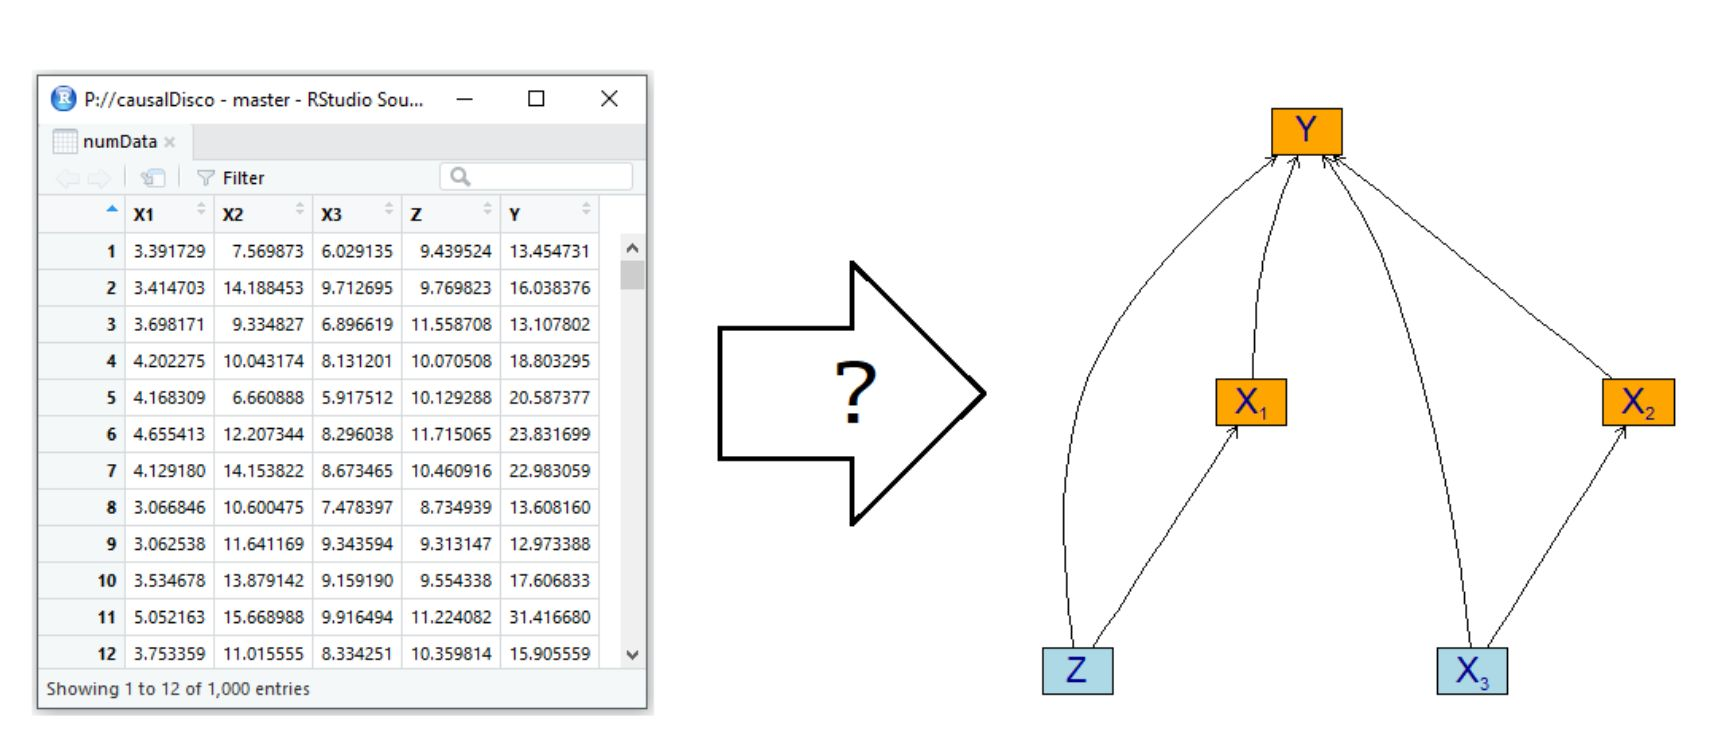
\includegraphics{../inst/images/Causality_fromData.jpg}

\href{https://github.com/annennenne/causalDisco/blob/master/slides/causaldisco_ahp_user2019.pdf}{CausalDisco}
an overview of methods to infer causal networks from data {]}

\begin{center}\rule{0.5\linewidth}{\linethickness}\end{center}

\hypertarget{study-types}{%
\section{Study Types}\label{study-types}}

.pull-left{[} \#\# Observational study - subjects are observed in order
to determine both their exposure and their outcome (e.g.~healthy,
cancer) - not randomized to the exposed or unexposed groups - The
exposure status is not determined by the researcher{]}

.pull-right{[} \#\# Experimental Intervention - experiment must be
repeatable - subjects are randomized to the exposed and unexposed
groups{]}

\begin{center}\rule{0.5\linewidth}{\linethickness}\end{center}

\hypertarget{study-types-1}{%
\section{Study Types}\label{study-types-1}}

.pull-left{[} \#\# Observational study - Case-control study - only
individuals with a specific characteristic (disease and similar
individuals without disease) - Cross-sectional study - aim to provide
data on the entire population under study - Longitudinal study -
repeated observations of the same variables (e.g., people) over short or
long periods of time{]}

.pull-right{[} \#\# Experiment Intervention - randomized controlled
trials{]}

\begin{center}\rule{0.5\linewidth}{\linethickness}\end{center}

\hypertarget{randomized-controlled-trial}{%
\section{Randomized controlled
trial}\label{randomized-controlled-trial}}

This year's Laureates have introduced a new approach to obtaining
reliable answers about the best ways to fight global poverty.

In brief, it involves \textbf{dividing this issue into smaller, more
manageable, questions} -- for example, the most effective interventions
for improving educational outcomes or child health.

They have shown that these smaller, more precise, questions are often
best answered via carefully \textbf{designed experiments} among the
people who are most affected.

.img-right{[} 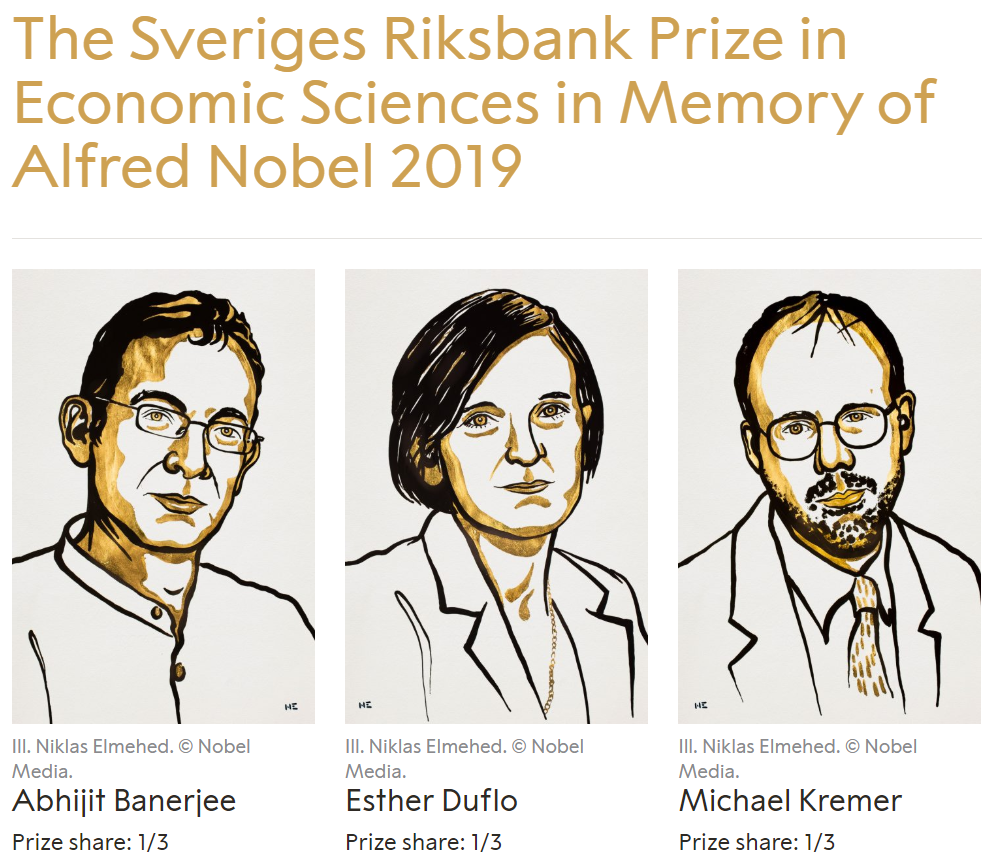
\includegraphics{../inst/images/Nobel2019.png}{]}

\hypertarget{randomized-controlled-trial-1}{%
\section{Randomized controlled
trial}\label{randomized-controlled-trial-1}}

Aims to reduce certain sources of \textbf{bias}

\begin{itemize}
\tightlist
\item
  Randomly allocate subjects to two or more groups
\item
  \emph{selection} and \emph{allocation} bias
\item
  Blinding
\item
  Information which may influence the participants is withheld until
  after the experiment is completed
\item
  A blind can be imposed on any participant of an experiment, including
  \textbf{subjects, researchers, technicians, data analysts, and
  evaluators}
\end{itemize}

\begin{center}\rule{0.5\linewidth}{\linethickness}\end{center}

\hypertarget{bias}{%
\section{Bias}\label{bias}}

What is \textbf{selection bias}?

--

sample obtained is \emph{not representative} of the population intended
to be analyzed

--

What is \textbf{allocation bias}?

--

\emph{systematic difference} in how participants are assigned to
treatment groups and comparison groups

\begin{center}\rule{0.5\linewidth}{\linethickness}\end{center}

\hypertarget{bias-1}{%
\section{Bias}\label{bias-1}}

Examples

\begin{itemize}
\tightlist
\item
  more care when processing treated samples than controls
\item
  \emph{adjusting} thresholds till obtaining significant results
\item
  ?
\end{itemize}

--

\hypertarget{how-could-you-improve-you-experiment-by-blinding}{%
\subsection{\texorpdfstring{How could you improve you experiment by
\emph{blinding}
?}{How could you improve you experiment by blinding ?}}\label{how-could-you-improve-you-experiment-by-blinding}}

\begin{itemize}
\tightlist
\item
  Do not transfer information unnecessary to perform a task, e.g.~use
  uninformative sample and group labels
\item
  Define analysis parameters beforhand
\end{itemize}

--

In clinical Trials double blind trials should be used where possible -
Single blind -- either patient or evaluator blind. - Double blind --
both patient and evaluator blind

\begin{center}\rule{0.5\linewidth}{\linethickness}\end{center}

\hypertarget{confounders}{%
\section{Confounders}\label{confounders}}

Correlation does not imply causation but causation may imply correlation

\textbf{Reichenbach's common cause principle:} A correlation occurs due
to one of the three possible mechanisms .img-small{[}
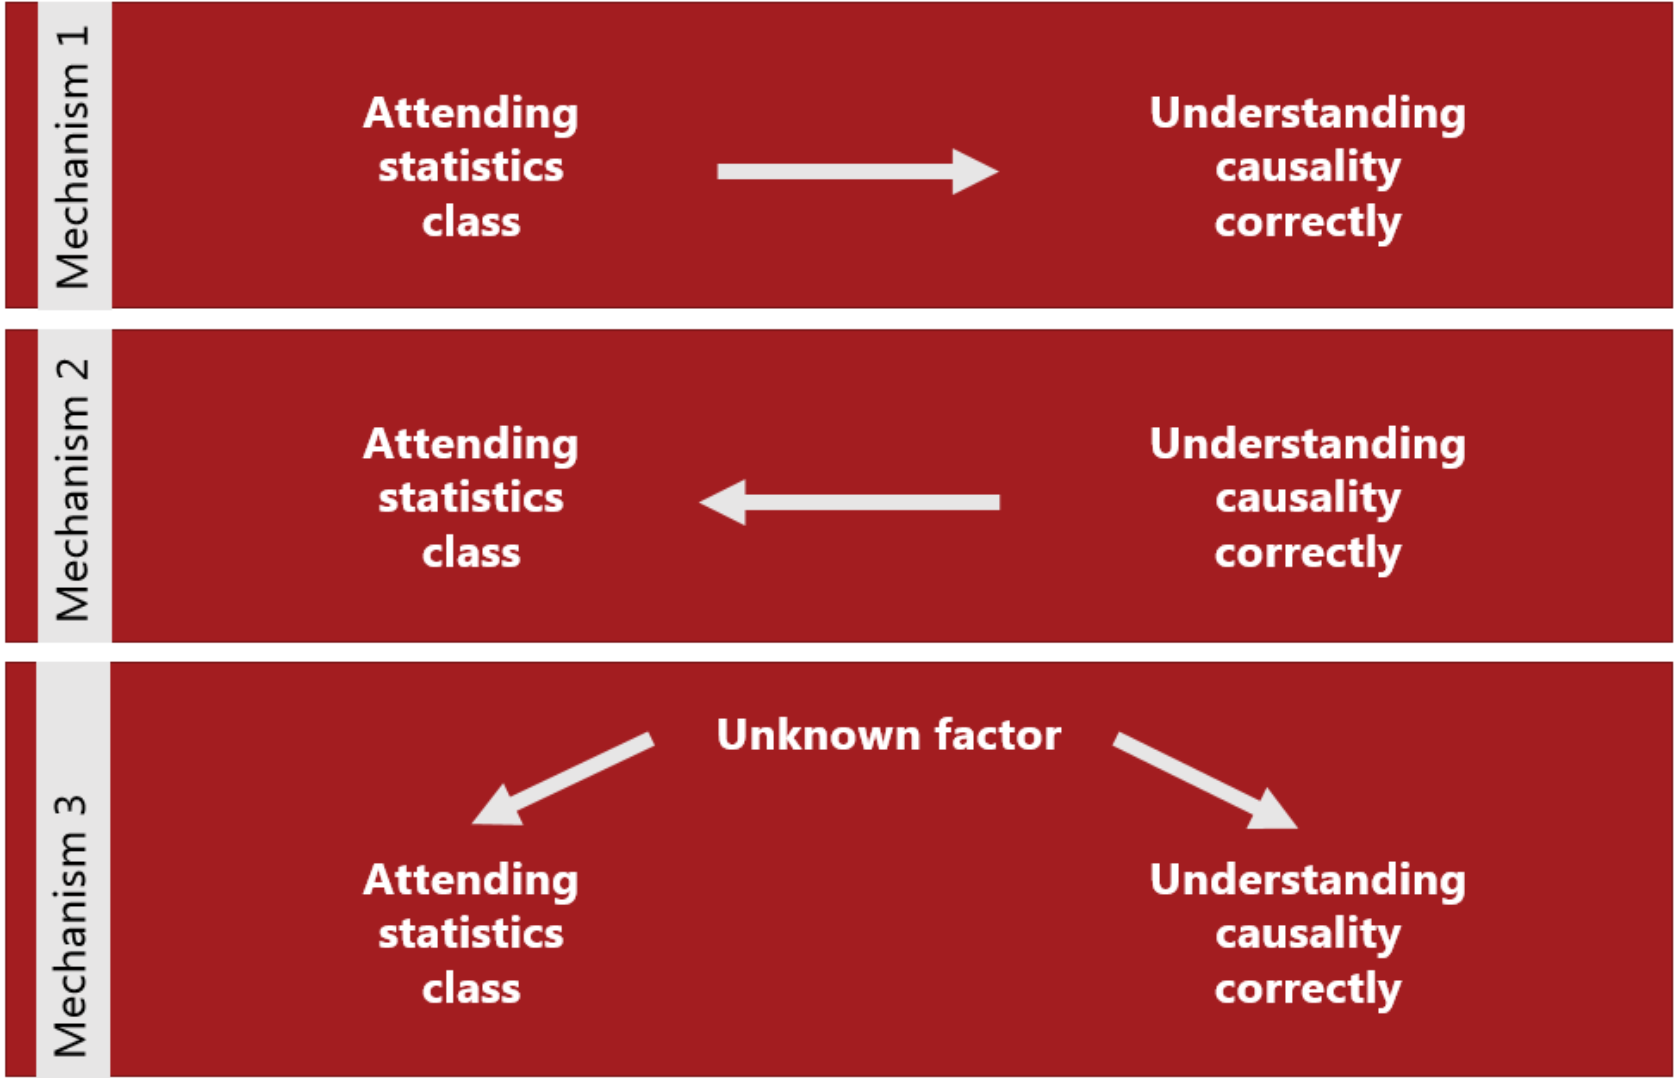
\includegraphics{../inst/images/Causality_Mechanisms_3.png}{]}

\textbf{Confounder} - is a variable that influences both the dependent
variable and independent variable, causing a spurious association.

\hypertarget{confounders-1}{%
\section{Confounders}\label{confounders-1}}

Document any possible co-variate, e.g.,

.pull-left{[}

\begin{itemize}
\tightlist
\item
  Human subjects:

  \begin{itemize}
  \tightlist
  \item
    age,
  \item
    bmi,
  \item
    gender,
  \item
    ethnicity,
  \item
    tissue,
  \item
    medical center {]}
  \end{itemize}
\end{itemize}

.pull-right{[} - Biochemical/Technical: - batch, - run Id - reagent lot
no, - chromatographic column, - name of technician, - instrument,{]}

\begin{center}\rule{0.5\linewidth}{\linethickness}\end{center}

\hypertarget{ethical-considerations}{%
\section{Ethical considerations}\label{ethical-considerations}}

\begin{itemize}
\item
  It is agreed that it is \textbf{unethical} \emph{to conduct research
  which is badly planned or executed}.
\item
  It is unethical to perform a trial which:
\item
  has many more subjects than are needed to reach a conclusion.
\item
  has little prospect of reaching any conclusion, e.g.~because of
  insufficient numbers of subjects (or some other aspect of poor design)
\item
  The local ethics committee has discretion on how it will supervise
  \textbf{non-interventional} studies

  \begin{itemize}
  \tightlist
  \item
    US - Institutional Review Board (IRB)
  \item
    EU - ethics committees
  \end{itemize}
\end{itemize}

\href{https://www.wma.net/policies-post/wma-declaration-of-helsinki-ethical-principles-for-medical-research-involving-human-subjects/}{Declaration
of Helsinki (1964+amendments))}

\begin{center}\rule{0.5\linewidth}{\linethickness}\end{center}

\hypertarget{types-of-error}{%
\section{Types of error}\label{types-of-error}}

A \emph{type I error} (false positive) occurs when the null hypothesis
(H0) is true, but is rejected. The \emph{type I error rate} or
\textbf{significance level} (p-Value) is the probability of rejecting
the null hypothesis given that it is true.

A \emph{type II error} (false negative) occurs when the null hypothesis
is false, but erroneously fails to be rejected. The \emph{the type II
error rate} is denoted by the Greek letter \(\beta\) and related to the
\textbf{power of a test} (which equals \(1−\beta\)).

For a given test, the only way to reduce both error rates is to
\textbf{increase the sample size}, and this may not be feasible.

.img-right{[} 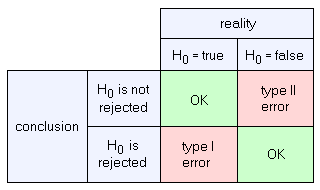
\includegraphics{../inst/images/hl_nullhypo_errors.png}{]}

\begin{center}\rule{0.5\linewidth}{\linethickness}\end{center}

\hypertarget{sample-size-calculation}{%
\section{Sample size calculation}\label{sample-size-calculation}}

.pull-left{[}

Run pilot experiment and measure the coefficient of variation (CV) or
\(\sigma^2\) of replicates:

\begin{itemize}
\tightlist
\item
  technical
\item
  \emph{biochemical}
\item
  \textbf{biological} {]}
\end{itemize}

.pull-right{[} - \emph{biological variance \textgreater{}\textgreater{}
bio-chem+tech variance} - Only provide biological replicates -
\emph{bio-chem+tech variance \textgreater{}\textgreater{} biological
variance} - \textbf{improve sample handling and preparation} - choose
different technology - buy better instrument{]}

\begin{center}\rule{0.5\linewidth}{\linethickness}\end{center}

\hypertarget{sample-size-calculations}{%
\section{Sample size calculations}\label{sample-size-calculations}}

.pull-left{[} For each statistical test, there exists a unique relation
between:

\begin{itemize}
\tightlist
\item
  desired smallest detectable effect size \(\mu\)
\item
  sample variance \(\sigma^2\)
\item
  sample size \(N\)
\item
  critical p-value \(p_0\)
\item
  statistical power {]}
\end{itemize}

.img-right{[}

\includegraphics[width=306px]{ExpDesign_files/figure-latex/unnamed-chunk-1-1}
\includegraphics[width=306px]{ExpDesign_files/figure-latex/unnamed-chunk-1-2}
{]}

\begin{center}\rule{0.5\linewidth}{\linethickness}\end{center}

\hypertarget{design}{%
\section{Design}\label{design}}

The key technical issue is whether comparisons are made \textbf{between}
or \textbf{within} subjects.

.pull-left{[} Between

\begin{itemize}
\tightlist
\item
  Parallel Group Design k - groups, \(n_i\) patients in group \(i\)
  receive treatment \(i\)
\item
  Factorial Design - more than one factor. combining treatments, e.g.~A
  and B to same patient. {]}
\end{itemize}

.pull-right{[} Within (repeated/paired)

\begin{itemize}
\tightlist
\item
  In series design each patient all \(k\) treatments in same order
\item
  crossover design each patient all \(k\) treatments in different order
  {]}
\end{itemize}

Are combinations of both possible?

\begin{center}\rule{0.5\linewidth}{\linethickness}\end{center}

\hypertarget{factorial-design-vs-parallel-group}{%
\section{Factorial Design vs Parallel
group}\label{factorial-design-vs-parallel-group}}

40 patients, Placebo, drug A and drug B.

How would you allocate these patients?

\begin{longtable}[]{@{}l@{}}
\toprule
\endhead
\begin{minipage}[t]{0.04\columnwidth}\raggedright
.pull-left{[} Factorial\strut
\end{minipage}\tabularnewline
\begin{minipage}[t]{0.04\columnwidth}\raggedright
- drug A + drug B 10 - plac A + drug B 10 - drug A + plac B 10 - plac A
+ plac B 10\strut
\end{minipage}\tabularnewline
\begin{minipage}[t]{0.04\columnwidth}\raggedright
Compare: - 20 drug A vs 20 plac A - 20 drug B vs 20 plac B {]}\strut
\end{minipage}\tabularnewline
\begin{minipage}[t]{0.04\columnwidth}\raggedright
.pull-right{[} Parallel\strut
\end{minipage}\tabularnewline
\begin{minipage}[t]{0.04\columnwidth}\raggedright
- drug A 13 - drug B 13 - plac 14\strut
\end{minipage}\tabularnewline
\begin{minipage}[t]{0.04\columnwidth}\raggedright
Compare: - 13 drug A vs 14 plac - 13 drug B vs 14 plac {]}\strut
\end{minipage}\tabularnewline
\bottomrule
\end{longtable}

layout: false

\hypertarget{interactions}{%
\section{Interactions}\label{interactions}}

An interaction may arise when considering the relationship among three
or more variables, and describes a situation in which the effect of one
causal variable on an outcome depends on the state of a second causal
variable.

--

\begin{itemize}
\tightlist
\item
  No interaction .img-right{[}
  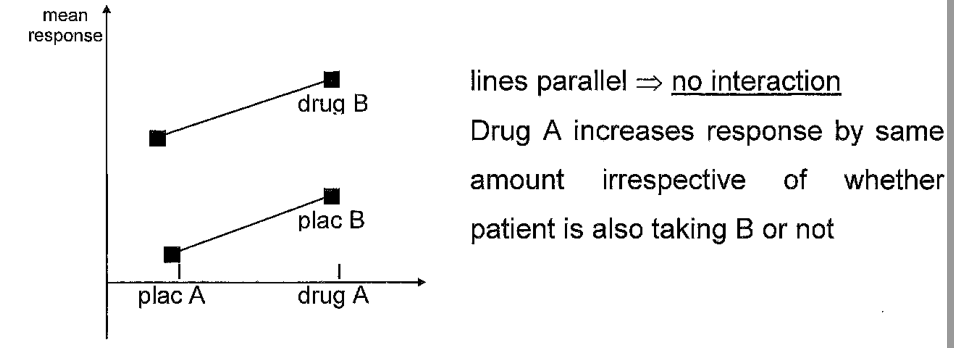
\includegraphics{../inst/images/TypesOfInteractions_NO.png}
\end{itemize}

{[}Medical Statistics - University of Sheffield{]} {]}

--

\begin{itemize}
\tightlist
\item
  Quantitative interaction
\end{itemize}

.img-right{[}
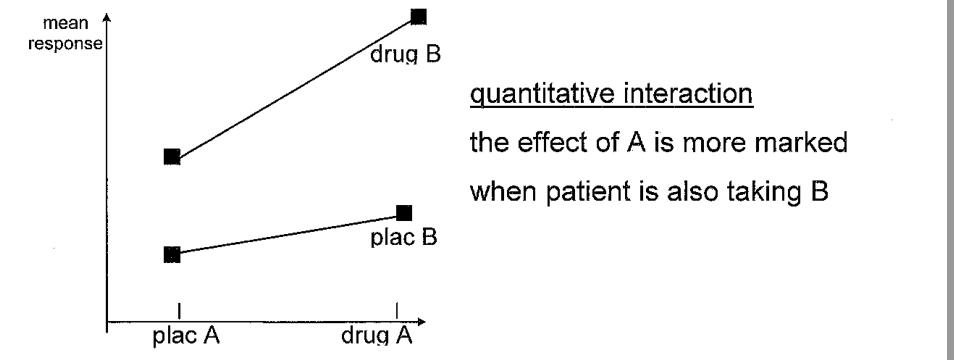
\includegraphics{../inst/images/TypesOfInteractions_Quanti.png}{]}

--

\begin{itemize}
\tightlist
\item
  Qualitative interaction
\end{itemize}

.img-right{[}
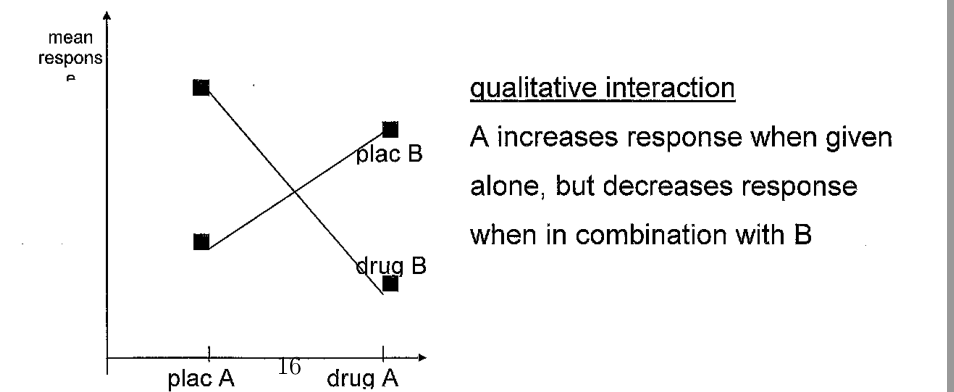
\includegraphics{../inst/images/TypesOfInteractions_Quali.png}{]}

\begin{center}\rule{0.5\linewidth}{\linethickness}\end{center}

\hypertarget{outlook---causality}{%
\section{Outlook - Causality}\label{outlook---causality}}

Assess whether a particular \textbf{agent}

caused or influenced a particular \textbf{outcome}

\(~\)

\(~\)

--

What would be the \textbf{agent} and \textbf{outcome} in label free
quantification?

--

\emph{agent} - medication or drug or treatment and confounding factors

\emph{outcome} - peptide and protein quantification values


\end{document}
